\chapter{Emotions and facial analysis}
\label{ch:literature-face}

The human face is a source of information and an important part of communication. Several elements connect this channel of information to emotional states, such as facial expressions and the activity of eyes and head \parencite{akakin2010spatiotemporal}. The analysis of such elements can convey information regarding emotional states, e.g. facial expressions are considered one of the most relevant features that can provide indication about emotional states \parencite{cowie2001emotion}.

\textcite{giannakakis2017stress} present a literature review focused on facial elements with value for detection of anxiety and stress, including the involvement of eyes (pupil size variations, gaze distribution, blinking rate), mouth (lips deformation, mouth activity) and head (head movement and velocity). Table \ref{table:stress-facial-features} lists all identified facial elements.

\begin{table}[h]
\begin{tabular}{lll}%
\toprule%
Head & Eyes & Mouth \\
\midrule
Head movement & Blink rate & Mouth shape \\
Skin color & Eyelid response & Lip deformation  \\
Hear rate (facial PPG) & Eye apperture & Lip corner puller \\
& Eyebrow movements & Lip corner depressor \\
& & Lip pressor \\
\midrule
Gaze & Pupil & \\
\midrule
Saccadic eye movements & Pupil size variation &  \\
Gaze spacial distribution & Pupil ratio variation &  \\
Gaze direction & &\\
\bottomrule%
\end{tabular}%
\caption{Categorization of facial elements connected with stress and anxiety \parencite{giannakakis2017stress}.}
\label{table:stress-facial-features}
\end{table}

There are indications that blinking increases with emotional arousal, including stress and anxiety levels \parencite{dinges2005optical}. Gaze direction, gaze congruence and the size of the gaze-cuing effect are also influenced by the level of anxiety or stress \parencite{staab2014influence}. Similarly mouth activity is influenced by conditions of stress, particularly lip movement \parencite{dinges2005optical} and asymmetric lip deformation \parencite{metaxas2004image}. Finally the frequency of mouth openenings has been measured as inversely proportional to the stress level under high cognitive load \parencite{liao2005decision}.

Different approaches have been used to connect facial analysis to emotional states of users. Initiatives include manual or automated face detection, use of machine learning models to map facial features to emotions and so on. The following sections present in more detail works related to face detection, including the approch used for analysis and connection to emotional states.

%%%%%%%%%%%%%%%%%%%%%%%%%%%%%%%%%%%%%%%%%%%%%%%%%%%%%%%%%%%%%%%%%%%%%%%%%%%%%%%%%%%%%%%%%%%%%%%%%%%%%%%
\section{Automated face detection}
%%%%%%%%%%%%%%%%%%%%%%%%%%%%%%%%%%%%%%%%%%%%%%%%%%%%%%%%%%%%%%%%%%%%%%%%%%%%%%%%%%%%%%%%%%%%%%%%%%%%%%%

A significant number of works in the literature use automated face dection techniques based on Computer Vision. Computer vision systems usually rely on image processing, artificial intelligence (e.g. machine learning) and decision making techniques to detect and classify objects from images or videos. A class of such objects is human faces, detected and analyzed by a process called facial alignment.

\begin{figure}[h]
    \centering
    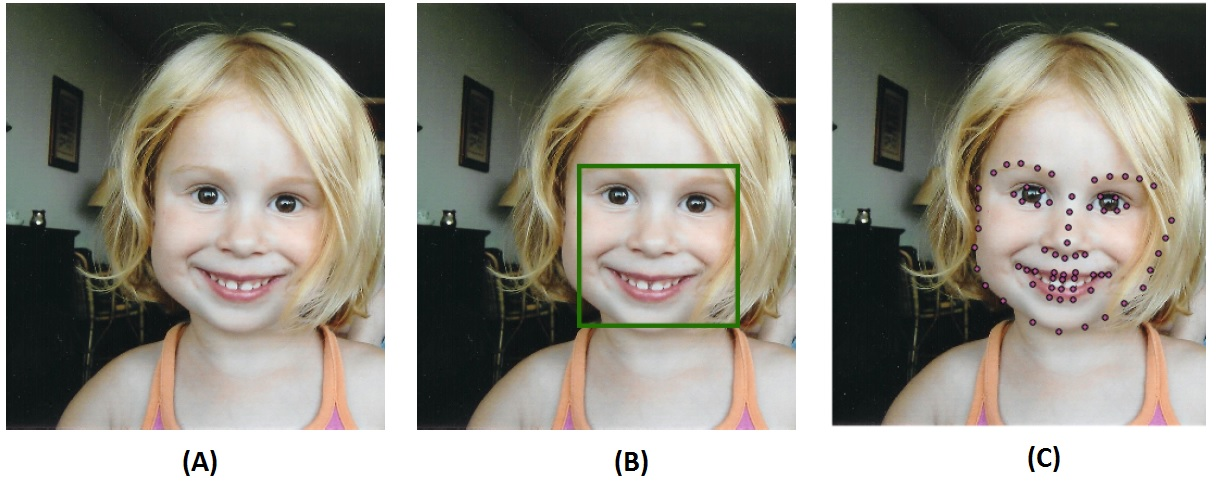
\includegraphics[width=\linewidth]{figures/face_alignment.jpg}
    \caption{Example of face alignment. (A) Input image. (B) Detected face. (C) Aligned face.}
    \label{fig:alignment}
\end{figure}

Facial alignment consists of identifying the position of specific features of the face, e.g. eye and nose, after the face has been detected in an image/video. Figure \ref{fig:alignment} demonstrates the process. This procedure is relevant in many different scenarios, for instance facial/expression recognition and pose estimation. Research has been conducted to create accurate and fast methods that can be used to perform face alignment under an ever growing set of challenging conditions, e.g. face movement combined with different lighting configurations.

Many methods have been proposed and a literature review shows that two basic approaches are widely used in alignment techniques: constrained local models and cascaded regression methods. Both approaches work on an image of a face contained within a rectangle obtained by a face detection algorithm, such as Viola \& Jones \parencite{viola2004robust}. The following sections describe each one of them, mentioning the most relevant techniques for facial alignment that are based on the approach being described.

\subsection{Constrained Local Model}

The Constrained Local Model (CLM) approach consists of locating a set of points on a target image, then applying a constrain to them. The constrain is usually based on a statistical shape model, which is obtained via training in a set of images featuring manually inserted landmarks. Since the shape model is statistical, the position of the points (landmarks) that it describes will always resemble a face, so proportions of lines and/or the distance among points will not be so different from a human face (at least not different from the ones found in the training set). Figure \ref{fig:clm-model-variation} illustrates the configuration of the shape model with different variations.

\begin{figure}[h]
    \centering
    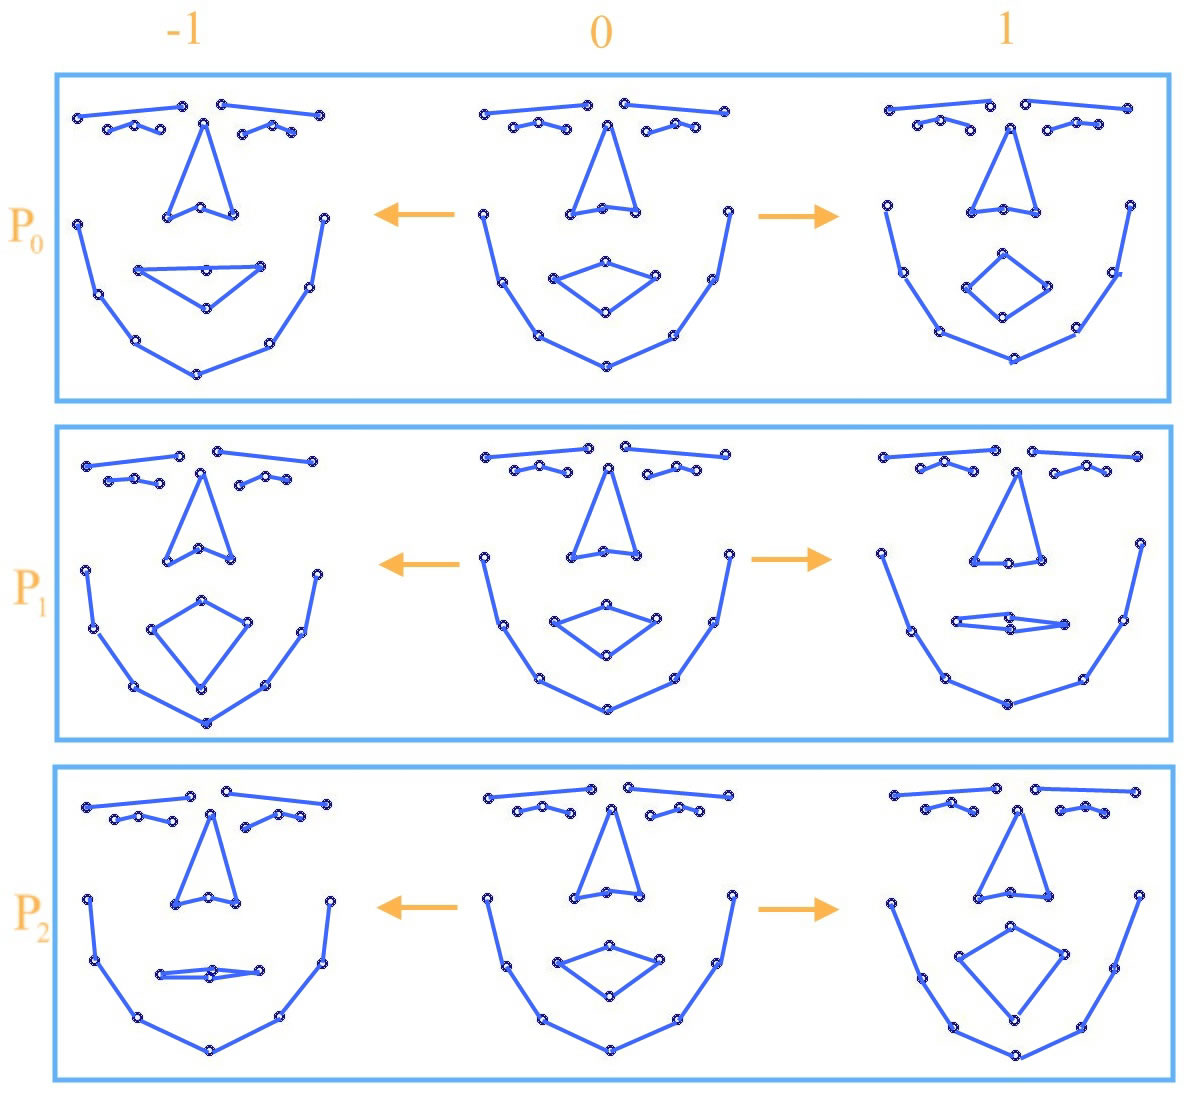
\includegraphics[width=0.5\linewidth]{figures/clm-model-variation.jpg}
    \caption{Configuration of the shape models with different variations \parencite{yu2010facial}.}
    \label{fig:clm-model-variation}
\end{figure}

Additionally to the shape model, there is a texture model that contains a set of patches (images) extracted from the training images by selecting the areas around the inserted landmarks. Those patches are used to guide the search procedure in the alignment process, which allows the technique to correctly identify the right model to properly align the face being analyzed. Figure \ref{fig:clm-patches} shows different shape models and their respective entries in the texture model.

The process of aligning a face is iterative and it starts by sampling points that are placed in the face image according to the current shape estimation of the face. In the first try, this estimation is usually the average face obtained from all training images. The area around the sampled points are extracted and used in a search to locate a set of similar patches in the texture model. The current shape estimation and the texture patches it locates are evaluated according to a cost function. As soon as the shape variation with the minimal cost is found, the process is repeated: new patches are sampled and searched against the texture model, the current estimation is adjusted and so on. Eventually the cost function will not produce a significantly different value from one iteration to another, which means the current estimation is the best match found.

\begin{figure}[h]
    \centering
    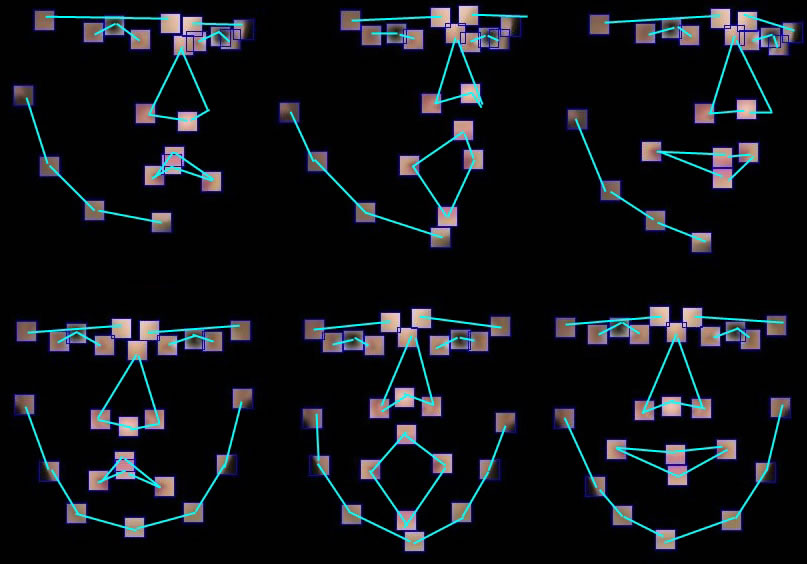
\includegraphics[width=0.6\linewidth]{figures/clm-patches.jpg}
    \caption{Shape models and their respective entries in the texture model \parencite{yu2010facial}.}
    \label{fig:clm-patches}
\end{figure}

Figure \ref{fig:clm-evolution} demonstrates the evolution of the technique as it iterates in an image. In Figure \ref{fig:clm-evolution}-(a), the mean shape is placed into the image and the patches are sampled around the (mistakenly) positioned landmarks. As the technique iterates ((b) and (c)), searched patches progressively induce changes in the current shape model, sampling more accurate patches. Eventually the technique converges to the aligned face, presented in Figure \ref{fig:clm-evolution}-(d).

\begin{figure}[h]
    \centering
    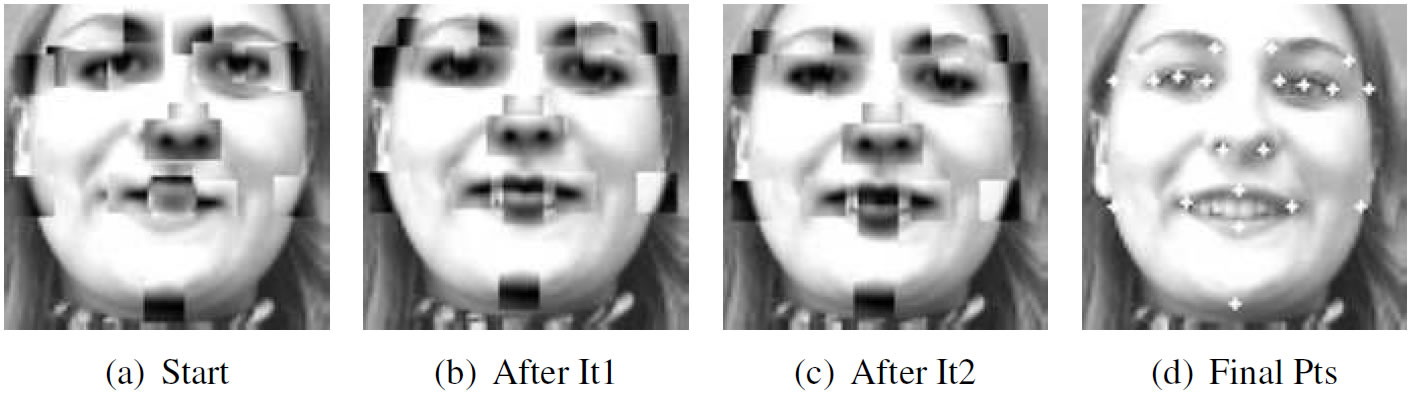
\includegraphics[width=\linewidth]{figures/clm-evolution.jpg}
    \caption{Iteration of CLM during the alignment of an image \parencite{cristinacce2006feature}.}
    \label{fig:clm-evolution}
\end{figure}

Two techniques that represent the CLM approach are the feature detection and tracking with constrained local models \parencite{cristinacce2006feature} and its 3D variation \parencite{baltruvsaitis20123d}, which uses 3D depth data to improve the process.

\subsection{Cascaded Regression}

The cascaded regression methods approach consists of using an initial guess shape that is progressively refined into the final answer (identification of key features in the image). This refinement is performed in a stage-by-stage manner (cascade) and the result of the current stage is used as the input for the next one. In each stage, the adjustment of the current shape (into the aligned result) is performed by a regression function, learnt via training. Early regressors in the cascade handle large variations in the shape, as opposed to the late ones, which focus on specific details. Each regressor extracts features from the image, which are then worked to produce variations in the current guess shape. The extracted features depend on the current shape and they are commonly referred as shape-indexed features.

The shape-indexed features are differences in pixel intensities. The calculation of a shape-indexed feature involves the selection of a few pixels and the subtraction of their intensities. The way those pixels are selected is usually different for each of the cascaded-regression techniques. Figure \ref{fig:shape-indexed} illustrates an example of selection of a few pixels for three particular landmarks. The landmark on the top-right (gray circle) highlights the selected pixels that will be used. The difference of intensities among those pixels will define this particular shape-indexed local feature. The shape-indexed local features are used in a decision process in each step (cascade), as illustrated by Figure \ref{fig:regressor-steps}. Usually the initial guess shape is the mean shape of the training set. This guess is used to calculate the current set of shape-indexed features to be extracted, which then guides the variation applied to the current shape. The variation to be applied is usually chosen based on the result of a cost function, which selects a variation that minimizes the distance between the current guess and the supposed aligned face. As the process repeats itself, different shape-indexed features are selected, a new variation is calculated and so on. Eventually the current shape will converge and it will represent the alignment for the face being analyzed (final shape estimation).

\begin{figure}[h]
    \centering
    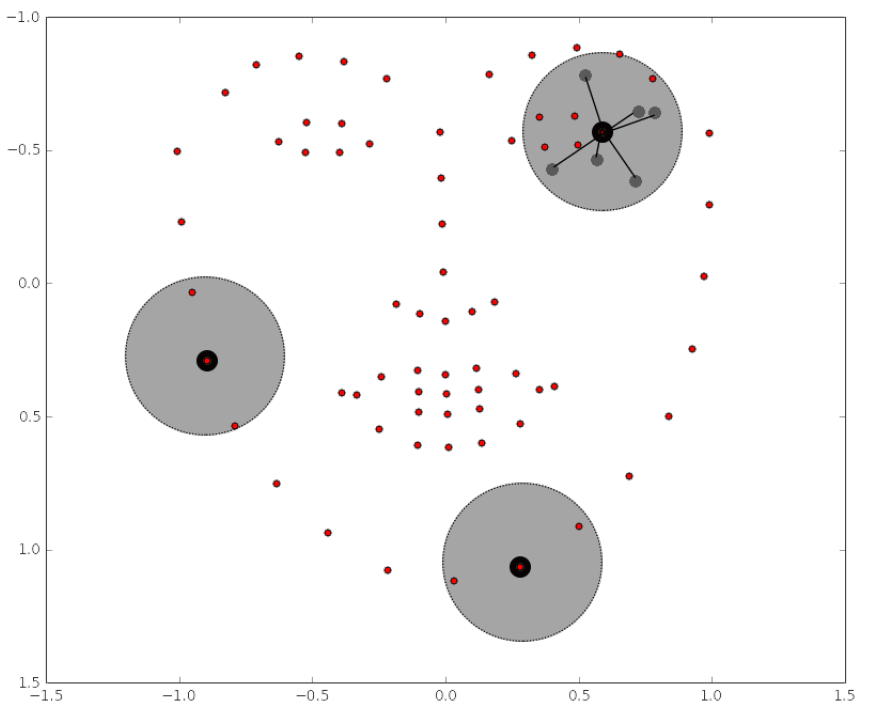
\includegraphics[width=0.5\linewidth]{figures/shape-indexed.png}
    \caption{Pixels used in the calculation of a shape-indexed feature \parencite{maris2015}.}
    \label{fig:shape-indexed}
\end{figure}

\begin{figure}[h]
    \centering
    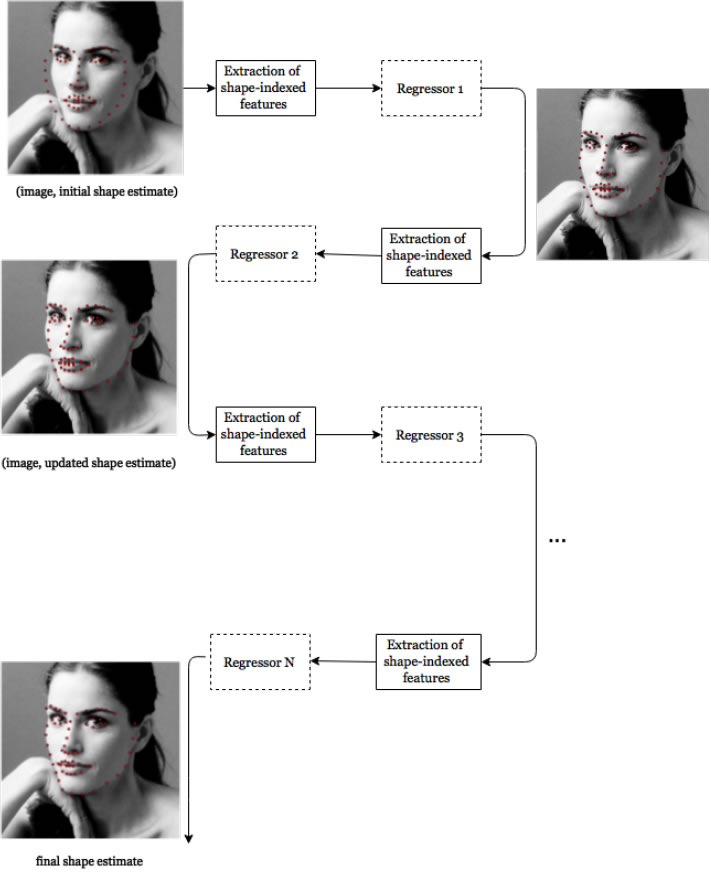
\includegraphics[width=0.9\linewidth]{figures/cascade-explanation.jpg}
    \caption{Estimation of face shape with regressors in a set of stages \parencite{maris2015}.}
    \label{fig:regressor-steps}
\end{figure}

Different variations are used to handle the training, the extraction of features and the way the regression is performed. The technique of face alignment with Ensemble of Regression Trees (ERT) \parencite{kazemi2014one}, for instance, estimates the face's landmarks by inputting the regressors with a sparse subset of pixels intensities, which is calculated with a prior probability on the distance of the pixels. The Supervised Descent Method (SDM) \parencite{xiong2013supervised}, on the other hand, extracts SIFT features from the current shape estimation and it converges the shape by solving a series of linear least square problems. The approach via regression of Local Binary Features (LBF) \parencite{ren2014face} proposes the use of a set of local binary features (opposed to a global view of the face) combined with a locality principle for learning and processing such features independently. Finally the face alignment by Explicit Shape Regression (ESR) \parencite{cao2014face} trains the regressors by explicitly minimizing the alignment error over training data, so all facial landmarks are regressed jointly.
%The regressors work by progressively inferring the shape, so the early regressors in the cascade handle large shape variations (ensures robustness) while later regressors focus on the small and subtle variations (ensures accuracy).

%%%%%%%%%%%%%%%%%%%%%%%%%%%%%%%%%%%%%%%%%%%%%%%%%%%%%%%%%%%%%%%%%%%%%%%%%%%%%%%%%%%%%%%%%%%%%%%%%%%%%%%
\section{Facial-based emotion prediction}
%%%%%%%%%%%%%%%%%%%%%%%%%%%%%%%%%%%%%%%%%%%%%%%%%%%%%%%%%%%%%%%%%%%%%%%%%%%%%%%%%%%%%%%%%%%%%%%%%%%%%%%

Works involving facial-based emotion prediction commonly focus on detecting or classifing emotional states based on the six basic emotions proposed by \textcite{ekman1971constants}, i.e. happiness, surprise, sadness, fear, anger and disgust. The process involves the mapping of such emotions from facial Action Units (AU), which are indentified according to schemes such as the Facial Action Coding System (FACS) \parencite{ekman1977facial,cohn2007observer}. FACS aims to standardize the measurements of facial expression by defining highly regulated procedural techniques to detect facial actions/movements, which are decomposed into 46 different AUs anatomically related to facial muscles. When analyzed in defined contexts, such mapped actions can present a correlation between determined facial features and emotional states, e.g. stress and boredom.

\begin{figure}[h!]
    \centering
    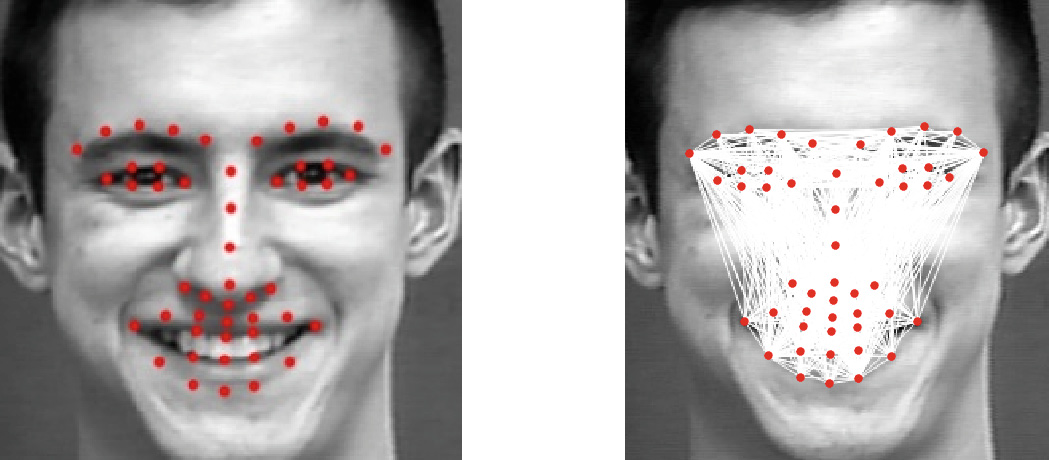
\includegraphics[width=\linewidth]{figures/samara2016sensing-distances.png}
    \caption{Distance-based facial feature descriptors. Left: detected facial landmarks. Right: highlight of the distance among facial landmarks. Reproduced from \parencite{samara2016sensing}.}
    \label{fig:distance-samara}
\end{figure}

\textcite{grafsgaard2013automatically} present an experiment where facial expression information is used to investigate emotional states. The experiment consists of an analysis of facial AUs during computer mediated tutoring sessions among students. Subjects and tutors interact through a tutoring software related to computer programming, while subjects are recorded. After each session, subjects answer a questionnaire related to measurements of cognitive load and engagement. The recordings are analyzed in an automated way with manual verification of the results. A predictive model is constructed using the questionnaire answers and the recording analysis, which results in correlations of facial AU and emotional states. The authors compare their findings against other research, which differ significantly. For instance, brow lowering has been correlated with confusion in previous work, however the authors found that it was a positive predictor of student frustration in the context of their experiment. \textcite{heylen2005facial} also present a similar investigation in a pilot experiment of a tutoring session related to the application of subcutaneous injection. Students interact with a virtual patient while using a physical haptic device to administrate an injection. The recordings of the students are analyzed by the researchers to make annotations of the expressions based on their own interpretation of the context. The researchers use a compilation of literature components to guide the evaluation of the collected data. As the authors point out, a variety of expressions occur, but most of the time students remain with a neutral facial expression. The annotated features are (ordered from most to less frequent): smile (total 22), raise eyebrows (11), pull down mouth corners (2) and frown (1).

%As opposed to previously mentioned works, our approach consists of using induced boring to stressful mechanics in games to produce variations in the emotional state of participants. Our experiment has a linear progression from a boring to a stressful state that should be perceived by the subjects. We believe such configuration gives our experiment a novel approach for the exploration of facial actions and HR regarding their connection to emotional states, since we can categorize information according to the induced (and theoretically known) emotional states. To the best of our knowledge, this is the first experiment where games with linear boring-to-stressful progression are used to deliberately induce emotional reactions.

Differently than the previously mentioned works, other initiatives aim to detect emotions based on the analysis of facial landmarks and their distances or movement. \textcite{joho2009exploiting} uses facial analysis for affective video summarisation. The authors use an automated face tracking approach to obtain a vector of motion features of certain regions of the face, named Motion Units (MU). MUs are classified by a Bayesian network, which is trained from labeled data. Results indicate promicing correlation between the manually annotated content of the videos and the automatically classified one. Somewhat similarly \textcite{akakin2010spatiotemporal} detects facial landmarks over consecutive frames of videos, whose trajectories (time series) during head gestures and facial expressions are organized in a spatiotemporal matrix. Discriminative features are extracted from the trajectory matrix, which are used to train machine learning models, i.e. Adaboost and SVM. Classification accuracy is reported to be around 90\% for the detection of 7 face and head gestures in a datased composed of 210 videos of 4 subjects). The detection of emotions, however, is limited to only two states, i.e. hapiness and sadness.

Finally \textcite{samara2016sensing} present the sensing of affective states based on the analysis of the distances of facial landmarks. Automated face detection is employed to detect facial landmarks, however no coding scheme is used to identify the detected points. Instead the authors use the Euclidian distance among facial landmarks, represented as distance vectors, to train a SVM model to detect expressions. Figure \ref{fig:distance-samara} illustrated the process. Detection accuracy is improved by a two-state SVM classification model, entitled by the authors as Hierarchical Parallelised Binary Support Machines (HPBSVM). Accuracy rates of about 96\% were achieved on two facial expression datasets.

%Such difference in results is expected due to the variational nature of facial expressions among different individuals and contexts, however it underlines the complexity of correlating facial features and emotions
